\documentclass[border=4pt,12pt]{standalone}
% House style for redrawn exam diagrams (diagram-v4: 0.4pt lines, filled -latex arrows, fine dashes; stipple and hatching drawn as real dots/lines (no PDF/SVG patterns, so they render in every browser and at any scale); transparent background). Every figure \input's this.
\usepackage{amsmath,amssymb}
\usepackage{txfonts}
\usepackage{pdfrender,xcolor}
% \halo{text}: label on shading. The shading stops just around each letter's outline (a thin knock-out that follows the
% glyphs, like the papers' typesetting), never a box. Owner: "I don't want a box around the text".
\newcommand{\halo}[1]{\leavevmode\rlap{\pdfrender{TextRenderingMode=2,LineWidth=2.2pt,LineJoinStyle=1,StrokeColor=white,FillColor=white}#1}#1}
\usepackage{tikz,pgfplots}
\pgfplotsset{compat=1.18}
\usetikzlibrary{arrows.meta,calc,angles,quotes,patterns,patterns.meta,intersections,positioning,decorations.markings,shapes.geometric}
% Stipple and hatching are drawn as actual dots / lines clipped to the region (path picture), NOT as pattern fills:
% SVG <pattern> fills vanish or blur when browsers scale the image, so the owner could not see the shading.
% Each dot is a 0.72pt square (keeps SVGs small; reads as a dot at print size). Dots sit on one global staggered grid, so neighbouring regions line up.
\makeatletter
\newdimen\ex@x \newdimen\ex@y \newdimen\ex@xa \newdimen\ex@ya \newdimen\ex@xb \newdimen\ex@yb \newcount\ex@row
\def\exam@stipplecolor{black!75}\def\exam@dotr{0.42pt}\def\exam@dotgap{2.5}
\def\ex@rowdots{\ifdim\ex@x<\ex@xb \pgfpathrectangle{\pgfqpoint{\dimexpr\ex@x-0.36pt\relax}{\dimexpr\ex@y-0.36pt\relax}}{\pgfqpoint{0.72pt}{0.72pt}}\advance\ex@x by \exam@dotgap pt\relax\expandafter\ex@rowdots\fi}
\def\exam@stipple{%
  \pgftransformreset% dots are sized in real points even inside scaled pictures
  \pgfpointanchor{path picture bounding box}{south west}\ex@xa=\pgf@x \ex@ya=\pgf@y
  \pgfpointanchor{path picture bounding box}{north east}\ex@xb=\pgf@x \ex@yb=\pgf@y
  \pgfsetfillcolor{\exam@stipplecolor}\pgfmathsetmacro\ex@h{\exam@dotgap/2}%
  \pgfmathtruncatemacro\ex@r{floor(\ex@ya/\ex@h)-1}\ex@row=\ex@r\relax
  \ex@y=\ex@r\dimexpr\ex@h pt\relax
  \loop\ifdim\ex@y<\ex@yb
    \pgfmathtruncatemacro\ex@c{floor(\ex@xa/\exam@dotgap)-1}\ex@x=\ex@c\dimexpr\exam@dotgap pt\relax
    \ifodd\ex@row \advance\ex@x by \ex@h pt\fi
    \ex@rowdots
    \advance\ex@y by \ex@h pt \advance\ex@row by 1
    \ifnum\numexpr\ex@row-(\ex@row/4)*4\relax=0 \pgfusepath{fill}\fi% flush every 4 rows: bounded TeX memory, few clip copies in the SVG
  \repeat\pgfusepath{fill}}
\newdimen\ex@d
\def\exam@hatch#1{% #1 = 1 for /, -1 for \ ; lines 45 degrees, 3pt apart
  \pgftransformreset
  \pgfpointanchor{path picture bounding box}{south west}\ex@xa=\pgf@x \ex@ya=\pgf@y
  \pgfpointanchor{path picture bounding box}{north east}\ex@xb=\pgf@x \ex@yb=\pgf@y
  \ex@d=\dimexpr\ex@yb-\ex@ya\relax \ex@x=\dimexpr\ex@xa-\ex@d\relax
  \loop\ifdim\ex@x<\ex@xb
    \ifnum#1>0 \pgfpathmoveto{\pgfqpoint{\ex@x}{\ex@ya}}\pgfpathlineto{\pgfqpoint{\dimexpr\ex@x+\ex@d\relax}{\ex@yb}}%
    \else \pgfpathmoveto{\pgfqpoint{\ex@x}{\ex@yb}}\pgfpathlineto{\pgfqpoint{\dimexpr\ex@x+\ex@d\relax}{\ex@ya}}\fi
    \advance\ex@x by 4.24pt
  \repeat
  \pgfsetlinewidth{0.4pt}\pgfsetstrokecolor{black}\pgfusepath{stroke}}
\def\examstipple{\exam@stipple}\def\examhatch{\exam@hatch}\def\examsetstipplecolor#1{\def\exam@stipplecolor{#1}}\def\examsetdotgap#1{\def\exam@dotgap{#1}}
\makeatother
% (legacy pattern kept for old files)
% staggered stipple like the NESA papers' dotted shading
\pgfdeclarepatternformonly{exam stipple}{\pgfpointorigin}{\pgfqpoint{2.2pt}{2.2pt}}{\pgfqpoint{2.2pt}{2.2pt}}{%
  \pgfpathcircle{\pgfqpoint{0.55pt}{0.55pt}}{0.42pt}\pgfpathcircle{\pgfqpoint{1.65pt}{1.65pt}}{0.42pt}\pgfusepath{fill}}
\tikzset{
  every picture/.style={line width=0.6pt, >={Latex[length=2mm,width=1.3mm]}},
  curve/.style={line width=0.6pt},
  open arrow/.style={-{Latex[length=2mm,width=1.3mm]}},  % owner: filled -latex heads everywhere, no open chevrons
  aux/.style={dash pattern=on 2pt off 1.5pt, line width=0.6pt},
  shade/.code={\def\exA{#1}\def\exB{none}\ifx\exA\exB\else\pgfkeysalso{fill=black!18}\fi},
  shade/.default=on,
  shade dots/.style={fill=none, path picture={\examstipple}},
  stipple color/.code={\examsetstipplecolor{#1}},
  stipple gap/.code={\examsetdotgap{#1}},
  shade dense dots/.style={fill=none, stipple gap=1.6, path picture={\examstipple}},
  shade hatch/.style={fill=none, path picture={\examhatch{1}}},
  shade hatch reverse/.style={fill=none, path picture={\examhatch{-1}}},
  shade solid/.style={fill=black},
  pt/.style={circle, fill, inner sep=1.1pt},
  open pt/.style={circle, draw, fill=white, inner sep=1.1pt},
}
\pgfplotsset{
  exam axes/.style={axis lines=middle, axis line style={->}, xlabel={$x$}, ylabel={$y$},
    xlabel style={anchor=west}, ylabel style={anchor=south}, tick label style={font=\small},
    every axis plot/.append style={line width=0.6pt, black}, samples=200, clip=false,
    enlargelimits=false, axis on top},
}

\begin{document}
% 571_q16_s1: solution: the question graph (scaled 0.6368 to the screenshot) with the sketch of y=f'(x)
% y=f(x) is a sketch (non-uniform x scale): traced from 571_q16_1 and refitted as one smooth spline (max dev 5.8 px);
% marked points (max, min, zeros, points at x=1 and x=9) are placed on the drawn curve (rule 16).
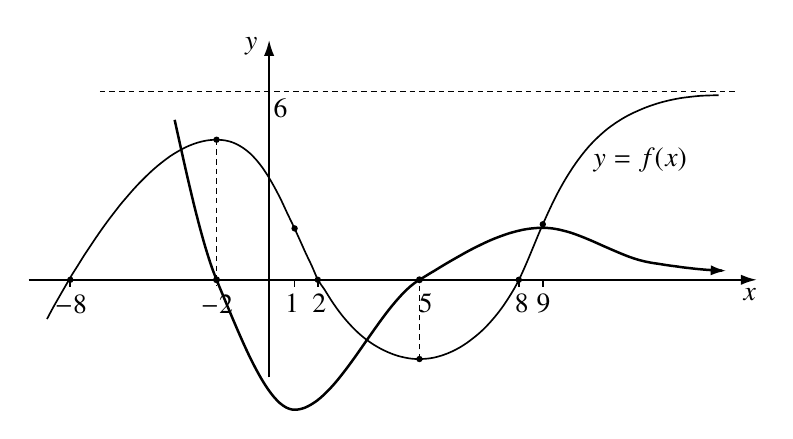
\begin{tikzpicture}[x=0.0127cm,y=-0.0127cm, every node/.style={font=\fontsize{10}{12}\selectfont}]
  \draw[aux] (138.1,71.5) -- (773.6,71.5);
  \draw[->] (66.8,260.0) -- (795.3,260.0);
  \draw[->] (307.5,357.7) -- (307.5,20.2);
  \draw[aux] (254.9,119.9) -- (254.9,266.7);
  \draw[aux] (457.9,339.3) -- (457.9,263.5);
  \draw (108.6,260.0) -- (108.6,267.3);
  \draw (333.0,260.0) -- (333.0,267.3);
  \draw (356.2,260.0) -- (356.2,267.3);
  \draw (557.3,260.0) -- (557.3,267.3);
  \draw (581.3,260.0) -- (581.3,267.3);
  \draw[line width=0.6pt] plot[smooth] coordinates {(85.3,299.3) (91.4,287.8) (97.6,276.9) (103.7,266.3) (109.9,255.6) (116.1,245.8) (122.2,236.0) (128.4,226.6) (134.6,217.4) (140.7,208.6) (146.9,200.1) (153.1,192.0) (159.2,184.2) (165.4,176.9) (171.5,169.9) (177.7,163.2) (183.9,157.0) (190.0,151.2) (196.2,145.8) (202.4,140.9) (208.5,136.4) (214.7,132.5) (220.9,129.0) (227.0,126.1) (233.2,123.7) (239.3,121.9) (245.5,120.6) (251.7,120.0) (257.8,120.0) (264.0,120.7) (270.2,122.3) (276.3,125.0) (282.5,128.8) (288.7,133.8) (294.8,140.2) (301.0,148.1) (307.1,157.4) (313.3,168.2) (319.5,180.2) (325.6,193.3) (331.8,206.2) (338.0,219.7) (344.1,233.3) (350.3,246.3) (356.5,260.4) (362.6,269.3) (368.8,279.2) (374.9,288.2) (381.1,296.4) (387.3,303.6) (393.4,310.0) (399.6,315.7) (405.8,320.6) (411.9,324.8) (418.1,328.4) (424.3,331.5) (430.4,334.1) (436.6,336.2) (442.7,337.7) (448.9,338.8) (455.1,339.3) (461.2,339.2) (467.4,338.7) (473.6,337.6) (479.7,335.9) (485.9,333.7) (492.0,331.0) (498.2,327.7) (504.4,323.8) (510.5,319.3) (516.7,314.3) (522.9,308.6) (529.0,302.1) (535.2,294.8) (541.4,286.6) (547.5,277.4) (553.7,267.1) (559.8,255.0) (566.0,241.0) (572.2,226.1) (578.3,211.4) (584.5,197.4) (590.7,184.1) (596.8,172.0) (603.0,160.9) (609.2,150.9) (615.3,141.9) (621.5,133.7) (627.6,126.4) (633.8,119.9) (640.0,114.1) (646.1,108.9) (652.3,104.4) (658.5,100.3) (664.6,96.7) (670.8,93.5) (677.0,90.7) (683.1,88.1) (689.3,85.8) (695.4,83.8) (701.6,82.0) (707.8,80.5) (713.9,79.2) (720.1,78.1) (726.3,77.3) (732.4,76.6) (738.6,76.0) (744.8,75.7) (750.9,75.5) (757.1,75.4)};
  \fill (108.6,260.0) circle (3.2);
  \fill (254.9,119.9) circle (3.2);
  \fill (333.0,208.6) circle (3.2);
  \fill (356.2,260.0) circle (3.2);
  \fill (457.9,339.3) circle (3.2);
  \fill (557.3,260.0) circle (3.2);
  \fill (581.3,204.5) circle (3.2);
  \node at (289.7,26.0) {$y$};
  \node at (787.6,275.0) {$x$};
  \node at (319.0,88.4) {$6$};
  \node at (109.5,284.5) {$-8$};
  \node at (255.6,284.5) {$-2$};
  \node at (330.4,283.9) {$1$};
  \node at (357.8,283.9) {$2$};
  \node at (464.2,283.9) {$5$};
  \node at (560.3,283.9) {$8$};
  \node at (582.0,283.9) {$9$};
  \node at (678.8,140.0) {$y=f(x)$};
  % y=f'(x) (teacher sketch, redrawn clean, black): zeros at x=-2 and x=5, min at x=1, max at x=9 (rules 16, 18);
  % heights and start/end from the sketch; teacher's dashed over-tracing of the x-axis and the scribbled loop left out (rule 17)
  \draw[->, line width=0.9pt] plot[smooth] coordinates {(213.0,100.0) (219.2,128.1) (225.4,155.6) (231.6,181.8) (237.8,206.2) (244.0,228.3) (250.2,247.6) (256.4,263.6) (262.6,278.6) (268.8,293.5) (275.0,308.1) (281.2,322.2) (287.4,335.6) (293.6,347.9) (299.8,359.1) (306.0,368.9) (312.2,377.1) (318.4,383.5) (324.6,387.8) (330.8,389.9) (337.0,389.7) (343.2,388.0) (349.4,384.9) (355.7,380.7) (361.9,375.4) (368.1,369.2) (374.3,362.3) (380.5,354.6) (386.7,346.5) (392.9,338.0) (399.1,329.2) (405.3,320.3) (411.5,311.5) (417.7,302.8) (423.9,294.4) (430.1,286.5) (436.3,279.2) (442.5,272.5) (448.7,266.7) (454.9,261.9) (461.1,258.1) (467.3,254.3) (473.5,250.6) (479.7,246.8) (485.9,243.1) (492.1,239.5) (498.3,236.0) (504.5,232.5) (510.7,229.2) (516.9,226.1) (523.1,223.1) (529.3,220.3) (535.5,217.8) (541.7,215.5) (547.9,213.4) (554.1,211.7) (560.3,210.2) (566.5,209.1) (572.7,208.4) (578.9,208.0) (585.1,208.1) (591.3,208.7) (597.5,209.8) (603.7,211.3) (609.9,213.1) (616.1,215.3) (622.3,217.7) (628.6,220.3) (634.8,223.0) (641.0,225.8) (647.2,228.5) (653.4,231.2) (659.6,233.8) (665.8,236.3) (672.0,238.5) (678.2,240.4) (684.4,241.9) (690.6,243.1) (696.8,244.0) (703.0,245.0) (709.2,245.9) (715.4,246.7) (721.6,247.6) (727.8,248.3) (734.0,249.0) (740.2,249.6) (746.4,250.1) (752.6,250.5) (758.8,250.8) (765.0,251.0)};
  \fill (254.9,260) circle (3.5); \fill (457.9,260) circle (3.5);
\end{tikzpicture}
\end{document}
